\chapter{Possible Future Work}
\label{chap:future}

The work in this thesis is pertinent to emerging methods in machine learning as well as current problems in structural bioinformatics.
As such, extensions of this work can be made in several distict veins, some focused on model formulation and training procedure, others on possible applications outside of interface prediction.
Several of these extensions are documented below, categorized as either extensions of method or extensions of application.

\section{Extensions of Method}

\subsection{Double Coupling and Ensemble Approaches}

As discussed in Chapter \ref{chap:experiments}, sum coupling outperforms product coupling on rigid and medium difficulty complexes, whereas product coupling is better for difficult complexes.
Therefore it would be reasonable to incorporate both sum and product coupling into a single convolution operation:

\begin{equation}
h_i(x | W^\textsc{c}, W^\textsc{n}, W^\textsc{e}, b) = \sigma \bigg( W^{\textsc{c}} x_i + \frac{1}{|\mathcal{N}_i|}\sum_{j \in \mathcal{N}_i} (W^{\textsc{n}} x_j) \odot (W^{\textsc{e}} A_{ij}) + W^{\textsc{n}} x_j + W^{\textsc{e}} A_{ij} + b \bigg),
\label{eq:double_coupling}
\end{equation}

\noindent
where here the same weight matrices are used in both the sum coupling and product coupling components to help prevent overfitting. 
Alternately, separate weight matrices could be used to increase the model's expressive power.

Recall that concerning the RFPP metric, the optimal network depth increased with complex difficulty, where more layers were needed for complexes of greater difficulty. 
This suggests that a ensemble model with multiple networks of varying depth could perform  better than each individual network.
Alternative ensemble approaches like \emph{boosting} or \emph{bagging} may also prove beneficial.
Boosting trains a sequence of "weak" models, with each added model being trained by giving more importance (loss weight) to examples misclassified by the existing set of models.
For interface prediction, this weighting can be performed on a per-complex basis, using RFPP or AUC as an indication of performance on each complex, or on a per-residue-pair basis, using the cross entropy loss of that specific training example.
The final prediction is a weighted average of the weak models' predictions, with the weights determined by the validation error of each respective model (with higher weight given to models with lower error).
Bagging creates multiple datasets by sampling with replacement from the original data set, and trains a different model on each sampled dataset.
This sampling can be performed at the complex level or the residue pair level.
Again, the final prediction is a weighted average of the weak models' predictions, weighted according to validation error.



\subsection{RFPP Optimization}

In practice, it may be more important to a biologist that a classifier give a single good prediction of the interface location, rather than predict the entire interface with a high degree of accuracy.
This was the original motivation for RFPP as a performance metric.
However, the existing model uses a loss function which incorporates every training example, not just the top positive prediction, hence the model is optimized for all examples.
It could be that optimizing the model for all examples sacrifices performance for the top predictions, and that directly optimizing RFPP could yield better results with respect to RFPP.
A modified version of the loss function is:

\begin{equation}
\mathbb{L}(\Theta | \{x_i, y_i\}) = - \max_{i} \big(y_{i1} f_1(x_i)\big),
\label{eq:rfpp_optimize}
\end{equation}

\noindent
which includes only the score of the maximum performing positive example.
Hence when the loss is minimized, the performance of the highest performing positive example will be maximized.
This loss function is not differentiable, but sub-gradient methods or differentiable alternatives exist which circumvent this limitation.
This method is currently being investigated by another student in Professor Ben-Hur's research group.

\subsection{Additional Data Sources}

The success of deep learning methods has been attributed to large volumes of data and deep architectures~\cite{krizhevsky2012}.
For interface prediction, despite the large volume of recorded protein structures, precious few complexes have been labeled in bound and unbound forms for use in model training and testing. 
This dependence on small curated subsets of the available proteins has potentially limited the full leveraging of deep learning methods, however some opportunities exist for enlarging the training and testing data.

The Docking Benchmark Dataset was conceived as a method to evaluate docking methods, and correspondingly was carefully constructed to be non-redundant with respect to SCOP families, in order to give a fair evaluation.
However for training purposes, it may be useful to include redundant proteins simply to provide the model with more training data. 
The Critical Assessment of PRediction of Interactions (CAPRI) is an annual competition aimed at evaluating protein-protein docking methods~\cite{janin2003}, and could also be used to help train or evaluate partner-specific protein interface prediction methods. 

\subsection{Unsupervised Pretraining}

Another approach to the problem of limited labeled complexes is to utilize the vast quantity (>125,000) of recorded protein structures via unsupervised pre-training.
Hinton and Salakhutdinov (2006)~\cite{hinton2006b} proposed a greedy layer-wise training algorithm for a particular form of neural network called an \emph{autoencoder}.
Training an autoencoder consists of training a sequence of Restricted Boltzmann Machines (RBMs) using unlabeled training data, then "unfolding" these RBMs into encoding and decoding layers which are intended to create a compressed representation of the input, before reconstructing the original input from the compressed representation.
The model weights can then be fine tuned using back propagation, where the output is further trained to reconstruct the input.
The encoding half of the autoencoder can be used independently of the decoding half to create compressed representations of the input that are often useful in supervised tasks like classification~\cite{hinton2006b, bengio2007}.

Masci et al (2011)~\cite{masci2011} proposed convolutional autoencoders (CAEs) which perform convolution to encode an image and \emph{deconvolution} to decode the image.
There is also a corresponding \emph{unpooling} operation which upsamples images which were pooled during the encoding step.
Deconvolution is simply a convolution operation performed on the result of an encoding convolution, with weights being tied between convolution and deconvolution layers.
For $k$ filters of size $m \times m$ and $c$ channels, the corresponding deconvolution would consist of $c$ filters of size $m \times m$ and $k$ channels, where the weights have been reflected in both spatial dimensions (e.g. the weights for the lower left pixel of the receptive field are now applied to the upper right pixel).
The spatial reflection allows a particular weight to carry a specific meaning, namely it characterizes the relationship between a particular pixel in an image and a pixel in its encoding.
To illustrate this, Figure \ref{fig:deconv} shows a deconvolution for a single filter and single channel.
CAEs are trained in the same greedy, layerwise fashion as conventional autoencoders.

\begin{figure}
	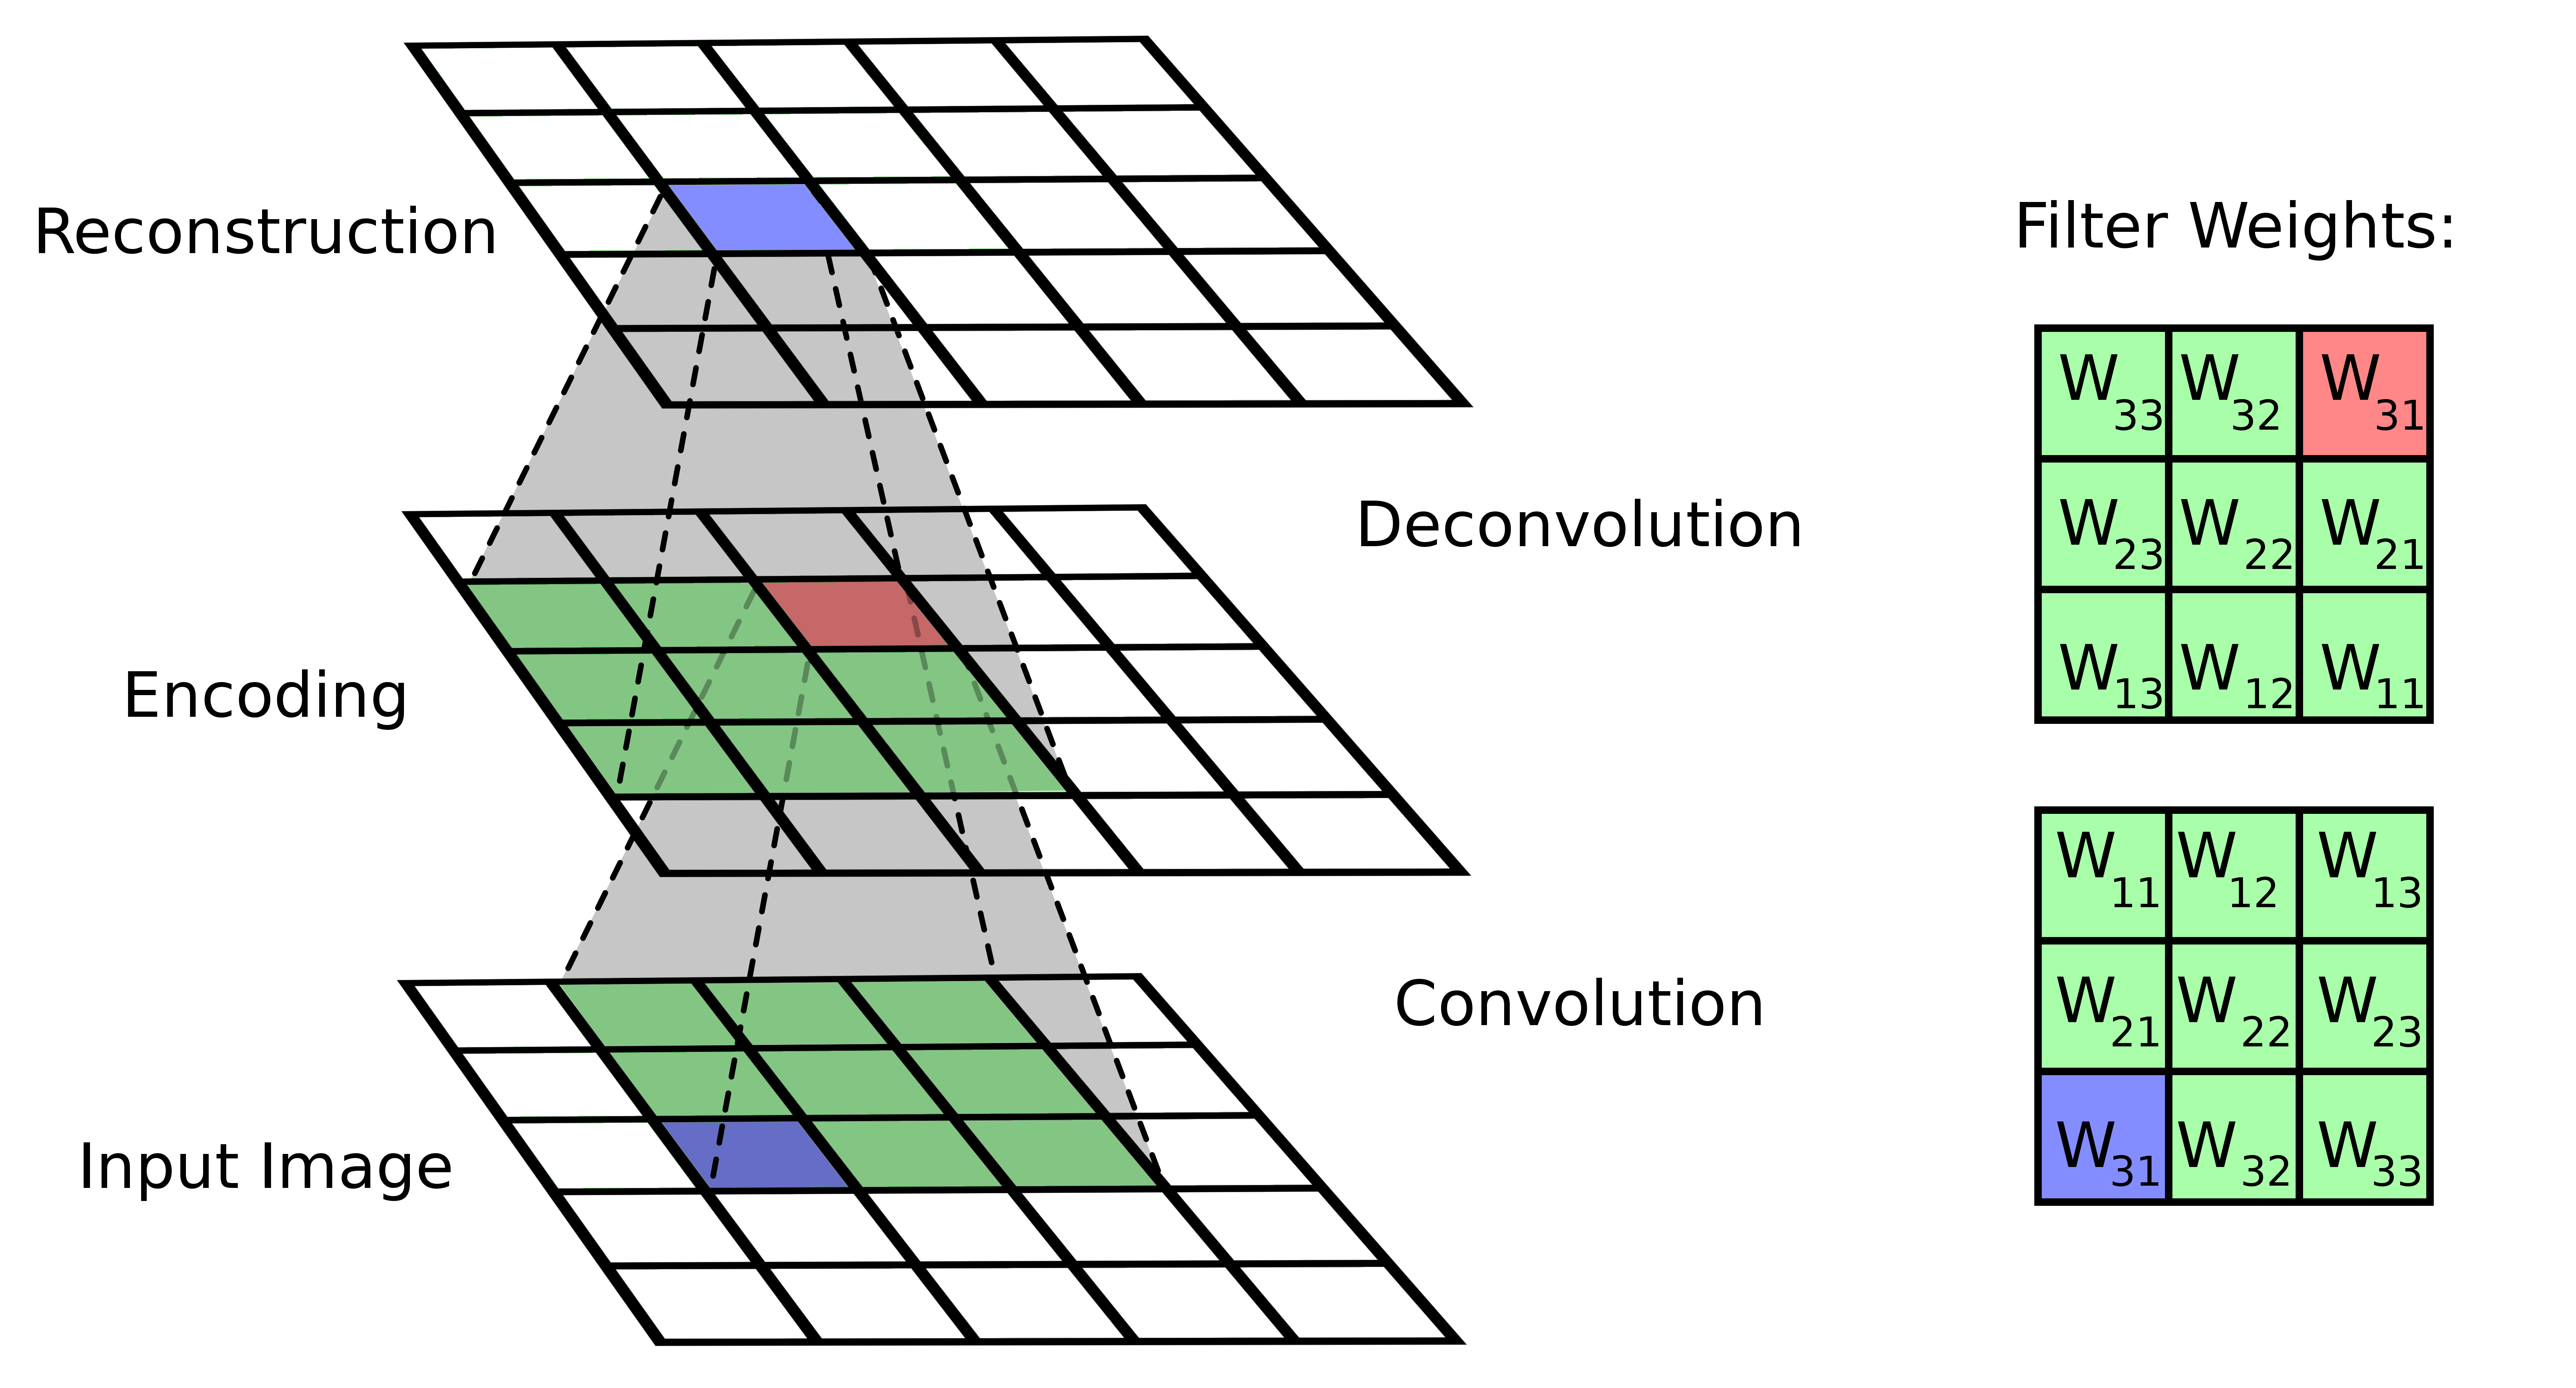
\includegraphics[width=0.8\textwidth]{conv_ae.png}
	\caption{Application of convolution, then deconvolution on a single channel input image. The relationship between the purple pixel in the input/reconstruction and the red pixel in the encoding is captured by the appropriate weight in the filters (lower left for convolution and upper right for deconvolution). By reflecting the convolution filter horizontally and vertically for use in deconvolution, the same weight ($W_{31}$) is used for this relationship during both encoding and decoding.
		\label{fig:deconv}}
\end{figure}


The concept of deconvolution can be applied to graph convolutions as well.
Note that when reflecting image convolution filters, the center weight remains in the same position.
In the same way, graph deconvolutions retain the same weights for the central vertex. 
Furthermore, since all neighbors use the same weights, there is no spatial reflection necessary.
Deconvolution simply consists of transposing the center and neighbor weight matrices so that channels become filters and filters become channels.
For sum coupling, deconvolution becomes:

\begin{equation}
\hat{x_i}(h_i | \tilde{W}^\textsc{c}, \tilde{W}^\textsc{n}, W^{\textsc{e}*}, b^*) = \sigma \bigg( \tilde{W}^{\textsc{c}} h_i + \frac{1}{|\mathcal{N}_i|}\sum_{j \in \mathcal{N}_i} (\tilde{W}^{\textsc{n}} h_j + W^{\textsc{e}*} A_{ij}) + b^* \bigg),
\label{eq:sum_deconv}
\end{equation}

\noindent
where $\hat{x}$ denotes the reconstruction of $x$ after deconvolving, $h_i$ is the convolved representation at vertex $i$, $\tilde{W}^\textsc{c}$ is the transpose of $W^\textsc{c}$, likewise for $\tilde{W}^\textsc{n}$ and $W^\textsc{n}$, and both $W^{\textsc{e}*}$ and $b^*$ are weight matrices with unshared weights. 
Note that graph convolutions generate representations on vertices of the graph, not the edges, so the non-encoded edge information ($A_{ij}$) must be used when deconvolving, and the weight matrix $W^{\textsc{e}*}$ cannot be tied to the encoding matrix $W^{\textsc{e}}$.

Alternately, edge representations could be created in a separate convolution operation, where an edge's receptive field is simply the incident vertices:

\begin{equation}
h_{ij}(A_{ij} |W^{\textsc{ee}}, W^{\textsc{ev}}, b_e) = \sigma\bigg( W^{\textsc{ee}} A_{ij} + \frac{1}{2}\big(
W^{\textsc{ev}} x_i + W^{\textsc{ev}} x_j \big) + b_\textsc{e} \bigg),
\label{eq:edge_conv}
\end{equation}

\noindent
where $h_{ij}$ is the representation of edge $(i, j)$ , $W^{\textsc{ee}}$ is the weight matrix associated with the edge, and $W^{\textsc{ev}}$ is the weight matrix associated with the incident vertices.
In this case, vertex deconvolution can use the encoded edge representations and associated weights.
Equation (\ref{eq:sum_deconv}) then becomes:

\begin{equation}
\hat{x_i}(h_i | \tilde{W}^\textsc{c}, \tilde{W}^\textsc{n}, \tilde{W}^\textsc{v}, b) = \sigma \bigg( \tilde{W}^{\textsc{c}} h_i + \frac{1}{|\mathcal{N}_i|}\sum_{j \in \mathcal{N}_i} (\tilde{W}^{\textsc{n}} h_j + \tilde{W}^{\textsc{ev}} h_{ij}) + b^* \bigg),
\label{eq:sum_deconv2}
\end{equation}

\noindent
where $\tilde{W}^{\textsc{V}}$ is the transpose of $W^{\textsc{V}}$.
Edges can also be deconvolved using the edge and vertex representations:

\begin{equation}
\hat{A_{ij}}(h_{ij} |\tilde{W}^{\textsc{ee}}, \tilde{W}^{\textsc{e}}, b) = \sigma \bigg( \tilde{W}^{\textsc{ee}} h_{ij} + \frac{1}{2}\big(
\tilde{W}^{\textsc{e}} h_i + \tilde{W}^{\textsc{e}} h_j \big) + b^{*}_\textsc{e} \bigg).
\label{eq:edge_conv}
\end{equation}

\noindent
This added weight sharing and symmetry between convolution and deconvolution operations may allow training of deeper networks which recognize more sophisticated structures.



\subsection{Simplicial Complex Convolution}

Graphs are only one way to model structural relationships between entities.
A simplicial complex is a generalization of a graph in which higher order simplices (triangles, tetrahedra, etc), in addition to edges, describe relationships between groups of vertices. 
For example, just as an edge indicates a relationship between two vertices, a triangle (or 2-simplex) indicates the relationship between three vertices.
For example, both the \v{C}ech and Vietoris-Rips definitions can be used to construct a simplicial complex from a set of points in an underlying metric space:

\begin{definition}
	Given a point set $X$ in some metric space and a number $\epsilon>0$, the \v{C}ech complex $C^{\textsc{\v{C}}}_\epsilon$ is the simplicial complex whose simplices are formed as follows. For each subset $S \subset X$ of points, form a ($\epsilon/2$)-ball around each point in $S$, and include $S$ as a simplex (of dimension $|S|$) if there is a common point contained in all of the balls in $S$.
\end{definition}

\begin{definition}
	Given a point set $X$ in some metric space and a number $\epsilon>0$, the Vietoris-Rips complex $C^{\textsc{VR}}_\epsilon$ is the simplicial complex whose simplices are formed as follows. For each subset $S \subset X$ of points, form a ($\epsilon/2$)-ball around each point in $S$, and include $S$ as a simplex (of dimension $|S|$) if for each pair of balls in $S$ there is a common point contained in both balls.
\end{definition}

In both definitions, simplices are included in the simplicial complex based on some notion of proximity.
This means simplicial complexes are naturally equipped to identify groups of neighbors in a neighborhood that are all close to one another, something which can be useful for interface prediction, where local regions of residues may constitute portions of an interface.
Though the number of possible convolution operations on simplicial complexes are many, one example is provided here for the purpose of discussion. 
In this formulation, rather than sum the signal from all neighbors in the receptive field, each simplex $S_k, k \in \{1, 2,... K\}$ (not counting vertices and edges, which are the lowest order simplexes) in the neighborhood is summed individually and the maximum simplex signal is added to the central signal:

\begin{equation}
\begin{split}
h_i(x |  & W^{\textsc{c}}, W^{\textsc{n}}, W^{\textsc{e1}}, W^{\textsc{e2}}, b) = \\ 
&\sigma \bigg( W^{\textsc{c}} x_i + \max_{k} \Big[ \frac{1}{|\mathcal{S}_k|}  \sum_{j \in \mathcal{S}_k} ( W^{\textsc{n}} x_j + W^{\textsc{e1}} A_{ij} ) + \frac{1}{|\mathcal{S}_k|^{2}}\sum_{j, l \in \mathcal{S}_k} (W^{\textsc{e2}} A_{jl}) \Big] + b \bigg).
\end{split}
\label{eq:simplicial_complex_conv}
\end{equation}

\noindent
This formulation also includes \emph{secondary} edges ($A_{jl}$), those between different neighbors in the same simplex.
It is possible that neighbors and edges occur in more than one simplex in the neighborhood, but that doesn't pose a problem because of the normalization and max function.
The use of simplicial complexes in defining convolution operations is currently being investigated by a student in Professor Ben-Hur's research group.


\section{Extensions of Application}

Interface prediction is not the only active area of protein research, and so the modeling of proteins and graphs and use of graph convolution could potentially be used for other protein problems as well.
A common characteristic of docking methods is that they create a high number of putative 3D bound structures~\cite{janin2013}.
The same pairwise neural network architecture used in this thesis could also be used to evaluate putative docking solutions and rank them in order of likelihood.
For example, the interface derived from a docking solution could be compared to the interface predicted by a trained pairwise graph convolutional neural network and ranked according to similarity with the network prediction.
Similarly, much research has been performed in protein modeling, which seeks to predict a protein's secondary and tertiary structures from sequence alone~\cite{schwede2013}.
Though graph convolutions cannot be used to create protein folds \emph{de novo}, they can be used to evaluate a set of putative folds and likewise rank them.
In both of these applications, regression is being performed not at the individual vertex level, but at the graph level.
These could take advantage of a global pooling method like taking the maximum or average across all vertices, or developing a \emph{fingerprint} similar to work by Duvenaud and Maclaurin, et al (2015)~\cite{duvenaud2015}.

Any application involving structured data that do not fit naturally into a grid is a potential candidate for graph convolutional approaches.
Aside from proteins, other biological and chemical data often meet this criterion.
In particular, Quantitative Structure-Activity Relationship (QSAR) and Quantitative Structure-Property Relationship (QSPR) both attempt to predict chemical behavior and properties of proposed chemical structures in order to identify structures with certain desired properties. 
Identified structures become candidates for laboratory synthesis and experimentation, a much more laborious and time consuming process. 
Studies in QSAR and QSPR have long been considered "unquestionably of great importance in modern chemistry and biochemistry"~\cite{karelson1996}.
Like proteins, chemical structures can be modeled as a graph and used to train graph convolutional networks to predict the properties of interest.
This is made possible by the vast and growing databases of chemical structures and their corresponding structures~\cite{olah2008, judson2008}.

Beyond the biochemical realm, graph structured data abound.
Knowledge bases are collections of structured data in the form of triples indicating \emph{(subject, predicate, object)}, where \emph{subject} and \emph{object} are named entities and \emph{predicate} indicates the relationship between them, and pairs indicating \emph{(subject, attribute)}, where \emph{attribute} is a type or property label for \emph{subject}.
These data can easily be thought of graphs, where entities are vertices each type of predicate is one of many different types of edge features, and each attribute is one of many different types of vertex features.
Knowledge bases emerge in online information repositories such as YAGO~\cite{mahdisoltani2014}, DBPedia~\cite{auer2007}, and Wikidata~\cite{vrandevcic2014}, and are used in the Google search engine \cite{singhal2012}.
Due to their large size, knowledge graphs are often under-annotated, where vertex relationships and properties are missing. 
A graph convolutional neural network can be used to predict properties or relationships on graphs, essentially performing automatic inference on the graph.



